\RequirePackage{iftex}
\ifPDFTeX
  \errmessage{This document requires XeLaTeX or LuaLaTeX. Please change your compiler.}
\fi
\documentclass[12pt]{report}

% @@@@@@@@@@@@@@@@@@@@@@@@@@@@@@@@@@@@@@@@@@@@@@@@@@@@@@@@@@@@>
% VALORES A MODIFICAR POR USTED:
% @@@@@@@@@@@@@@@@@@@@@@@@@@@@@@@@@@@@@@@@@@@@@@@@@@@@@@@@@@@@>

% NOTE: Leer nota en el README sobre la font.

\newcommand{\titulo}{Título de la memoria}
\newcommand{\ciudad}{Valparaíso} % e.g. Valparaíso
% TODO: Consultar el formato de los nombres:
\newcommand{\nombrealumno}{Sebastian Salgado Polanco}
\newcommand{\nombreprofesor}{Daniela Opitz}
\newcommand{\nombrecorreferente}{Marylin Cruces}
% Mes y año del examen
\newcommand{\mesexamen}{Diciembre}
\newcommand{\anioexamen}{2025}
% Dedicatoria y agradecimientos
\newcommand{\dedicatoria}{
Considerando lo importancia de este trabajo para los alumnos, este apartado es para que el autor entregue palabras personales para dedicar este documento. La extensión puede ser de máximo una hoja y se deben mantener este formato, tipo y tamaño de letra.
}
\newcommand{\agradecimientos}{
Considerando la importancia de este trabajo para los alumnos, este apartado se podrá incluir en el caso de que el autor desee agradecer a las personas que facilitaron alguna ayuda relevante en su trabajo para la realización de este documento. La extensión puede ser de máximo una hoja y se deben mantener este formato, tipo y tamaño de letra.
}
\newcommand{\resumen}{
El resumen y las palabras clave no deben superar la mitad de la página, donde debe precisarse brevemente: 1) lo que el autor ha hecho, 2) cómo lo hizo (sólo si es importante detallarlo), 3) los resultados principales, 4) la relevancia de los resultados. El resumen es una representación abreviada, pero comprensiva de la memoria y debe informar sobre el objetivo, la metodología y los resultados del trabajo realizado.
}
\newcommand{\resumeningles}{
Corresponde a la traducción al idioma inglés del Resumen anterior. Sujeto a la misma regla de extensión del Resumen.
}
\newcommand{\palabrasclave}{
Cinco es el máximo de palabras clave para describir los temas tratados en la memoria, ponerlas separadas por punto y comas.
}
\newcommand{\palabrasclaveingles}{
Corresponde a la traducción al idioma inglés de Palabras Clave anteriores.
}
% @@@@@@@@@@@@@@@@@@@@@@@@@@@@@@@@@@@@@@@@@@@@@@@@@@@@@@@@@@@@>

% Paquete para importar imágenes
\usepackage{graphicx}
% Directorio de las imágenes
\graphicspath{ {figures/} }

% Idioma y fuentes
\usepackage[spanish,es-tabla]{babel}
\usepackage[T1]{fontenc}

\usepackage{fontspec}
% Selección robusta de fuente principal con respaldo en Windows
\newcommand{\MainFontName}{Carlito}
\IfFontExistsTF{Carlito}{
  \renewcommand{\MainFontName}{Carlito}
}{
  \IfFontExistsTF{Calibri}{
    \renewcommand{\MainFontName}{Calibri}
  }{
    \renewcommand{\MainFontName}{Latin Modern Roman}
  }
}
\setmainfont{\MainFontName}[BoldFont={* Bold}, ItalicFont={* Italic}]

% Paquete para definir cualquier tamaño de font
\usepackage{anyfontsize}

% Tamaño de la página y márgenes
\usepackage[letterpaper,top=2.5cm,bottom=3cm,left=3cm,right=3cm,marginparwidth=1.75cm]{geometry}

% Determinar interlineado:
\renewcommand{\baselinestretch}{1.0}

% Eliminar sangrías:
\setlength{\parindent}{0cm}

% Paquete para definir los formatos de los títulos
\usepackage[explicit]{titlesec}

\titleformat{name=\section}[block]{\fontsize{16}{24}\selectfont\bfseries}{}{0pt}{#1}
\titleformat{name=\section,numberless}[block]{\fontsize{16}{24}\selectfont\bfseries}{}{0pt}{#1}
\titlespacing*{name=\section}{0pt}{0pt}{0.5cm}
\titlespacing*{name=\section,numberless}{0pt}{0pt}{0.5cm}

% Separación entre parrafos
\setlength{\parskip}{0.4cm}

% Paquetes de utilidad general
\usepackage{amsmath}
\usepackage{graphicx}
\usepackage{float}
\usepackage[colorlinks=true, allcolors=blue]{hyperref}

% Formato de las tablas de contenido
\usepackage{tocbasic}

%% Originalmente se usaba tocstyle en vez de tocbasic.
%% Si se quiere usar, descomentar:
% \usepackage[tocflat]{tocstyle}
% \usetocstyle{allwithdot}
%% tocstyle.sty se obtener de https://github.com/firemodels/fds/blob/master/Manuals/LaTeX_Style_Files/tocstyle.sty

% Para obtener el número de la última página
\usepackage{lastpage}

% Header y footer
\usepackage{fancyhdr}
\fancypagestyle{portada}{
    \lhead{}
    \chead{}
    \rhead{}
    \lfoot{}
    \cfoot{\fontsize{10}{12}\selectfont \thepage}
    \rfoot{}
    \renewcommand{\headrulewidth}{0pt}
}
\fancypagestyle{intermedio}{
    \lhead{}
    \chead{\fontsize{10}{12}\selectfont\MakeUppercase{\titulo}}
    \rhead{}
    \lfoot{}
    \cfoot{\fontsize{10}{12}\selectfont Página \textbf{\thepage}\ de \textbf{\pageref{LastPage}}}
    \rfoot{}
    \renewcommand{\headrulewidth}{1pt}
}

% Comandos para secciones
\newcommand{\secnumbersection}[1]{
\addtocounter{section}{1}
\phantomsection
\section*{CAPÍTULO \thesection \texorpdfstring{\\}\ #1}
\addcontentsline{toc}{section}{CAPÍTULO \thesection : #1}
\setcounter{subsection}{0}
}
\newcommand{\secnumberlesssection}[1]{
\section*{#1}
\phantomsection
\addcontentsline{toc}{section}{#1}
\setcounter{subsection}{0}
}

% Nombres
\addto\captionsspanish{\renewcommand{\contentsname}{ÍNDICE DE CONTENIDOS}}
\addto\captionsspanish{\renewcommand{\listfigurename}{ÍNDICE DE FIGURAS}}
\addto\captionsspanish{\renewcommand{\listtablename}{ÍNDICE DE TABLAS}}
\makeatletter
\renewenvironment{thebibliography}[1]
     {\secnumberlesssection{REFERENCIAS BIBLIOGRÁFICAS}
      \@mkboth{\MakeUppercase\bibname}{\MakeUppercase\bibname}%
      \list{\@biblabel{\@arabic\c@enumiv}}%
           {\settowidth\labelwidth{\@biblabel{#1}}%
            \leftmargin\labelwidth
            \advance\leftmargin\labelsep
            \@openbib@code
            \usecounter{enumiv}%
            \let\p@enumiv\@empty
            \renewcommand\theenumiv{\@arabic\c@enumiv}}%
      \sloppy
      \clubpenalty4000
      \@clubpenalty \clubpenalty
      \widowpenalty4000%
      \sfcode`\.\@m}
     {\def\@noitemerr
       {\@latex@warning{Empty `thebibliography' environment}}%
      \endlist}
\makeatother

% Personalizar Tabla de Contenidos

\usepackage{tocloft}
\renewcommand{\cftsecfont}{\fontsize{12}{14}\selectfont\fontspec{\MainFontName}}
\renewcommand{\cftsubsecfont}{\fontsize{12}{14}\selectfont\fontspec{\MainFontName}}
\renewcommand{\cftsubsubsecfont}{\fontsize{12}{14}\selectfont\fontspec{\MainFontName}}

\renewcommand\cftfigfont{\fontsize{12}{14}\selectfont\fontspec{\MainFontName}}

% Links sin color
\usepackage{hyperref}
\hypersetup{colorlinks = false}

% Comando para secciónes sin enumeración
% (sugerido por @anibalbastiass https://github.com/autopawn/tex-thesis-template/issues/5#issuecomment-916106128)
\newcommand{\secnumberlesssubsection}[1]{
\subsection*{#1}
\phantomsection
\addcontentsline{toc}{subsection}{#1}
\setcounter{subsection}{0}
}
% Forma de uso:
% \secnumberlesssubsection{"Sub seccion sin enumeración"}

% @@@@@@@@@@@@@@@@@@@@@@@@@@@@@@@@@@@@@@@@@@@@@@@@@@@@@@@@@@@@>
\begin{document}
\sloppy % Para evitar que referencias se escapen de los márgenes.

\pagestyle{portada}
\pagenumbering{roman}
% NOTE: Este archivo contiene la portada, la dedicatoria, los agradecimientos y el resumen.
% __NO ES NECESARIO MODIFICAR ESTE ARCHIVO__, esas se modifican con los comandos que aparecen en main.tex
%@@@@@@@@@@@@@@@@@@@@@@@@@@@@@@@@@@@@@@@@@@@@@@@@@@@@@@@@@@@@@@
\begin{titlepage}
\begin{center}
\noindent
{\fontsize{18}{22}\selectfont UNIVERSIDAD TÉCNICA FEDERICO SANTA MARÍA \\}
{\fontsize{16}{19}\selectfont DEPARTAMENTO DE INFORMÁTICA \\}
{\fontsize{16}{19}\selectfont \MakeUppercase{\ciudad}\ - CHILE \\}
\vspace{1.5cm}

\includegraphics[width=4.41cm,height=3.34cm]{logo/logo.jpg} \\
\vspace{1.5cm}
{\fontsize{20}{24}\selectfont ``\MakeUppercase{\titulo}'' \\}
\vfill
{\fontsize{16}{19}\selectfont \MakeUppercase{\nombrealumno} \\}
\vfill
{\fontsize{16}{19}\selectfont MEMORIA PARA OPTAR AL TÍTULO DE \\}
{\fontsize{16}{19}\selectfont INGENIERO CIVIL EN INFORMÁTICA \\}
\vspace{1.5cm}
{\fontsize{14}{17}\selectfont Profesor Guía: \nombreprofesor \\}
{\fontsize{14}{17}\selectfont Profesor Correferente: \nombrecorreferente \\}
\vspace{2.5cm}
{\fontsize{14}{17}\selectfont \mesexamen\ - \anioexamen \\}
\end{center}
\end{titlepage}

%@@@@@@@@@@@@@@@@@@@@@@@@@@@@@@@@@@@@@@@@@@@@@@@@@@@@@@@@@@@@@@
\newpage
\setcounter{page}{2}
\
\vfill
\vfill
\begin{flushright}
\noindent {\fontsize{16}{19}\selectfont \textbf{DEDICATORIA} \\}
\end{flushright}
\begin{flushright}
\noindent \dedicatoria
\end{flushright}
\vfill
%@@@@@@@@@@@@@@@@@@@@@@@@@@@@@@@@@@@@@@@@@@@@@@@@@@@@@@@@@@@@@@
\newpage
\begin{center}
\noindent {\fontsize{16}{19}\selectfont \textbf{AGRADECIMIENTOS} \\}
\end{center}
\noindent \agradecimientos
\vfill
%@@@@@@@@@@@@@@@@@@@@@@@@@@@@@@@@@@@@@@@@@@@@@@@@@@@@@@@@@@@@@@
\newpage
\secnumberlesssection{RESUMEN}
\vspace{0.3cm}
\noindent \textbf{Resumen---}\resumen \ \\
\vspace{0.3cm} \\
\noindent \textbf{Palabras Clave---}\palabrasclave \ \\
% @@@@@
\vspace{1.2cm} \\
% @@@@@
%\noindent {\fontsize{16}{19}\selectfont \textbf{ABSTRACT}}
%\vspace{1.2cm} \\
\secnumberlesssection{ABSTRACT}
\vspace{0.3cm}
\noindent \textbf{\emph{Abstract}---}\resumeningles \ \\
\vspace{0.3cm} \\
\noindent \textbf{\emph{Keywords}---}\palabrasclaveingles \ \\
%@@@@@@@@@@@@@@@@@@@@@@@@@@@@@@@@@@@@@@@@@@@@@@@@@@@@@@@@@@@@@@


\newpage
\secnumberlesssection{GLOSARIO}

Aquí se deben colocar las siglas mencionadas en el trabajo y su explicación, por orden alfabético. Por ejemplo: \\

{\setlength{\parskip}{0cm} % Para evitar saltar entre cada elemento nombrado.
%Colocar aquí siglas:
DI: Departamento de Informática.

UTFSM: Universidad Técnica Federico Santa María.
}


%Índice de contenidos:
\newpage
\thispagestyle{portada}
\tableofcontents

%Índice de figuras:
\newpage
\thispagestyle{portada}
\phantomsection
\addcontentsline{toc}{section}{ÍNDICE DE FIGURAS}
\listoffigures
\phantomsection
\addcontentsline{toc}{section}{ÍNDICE DE TABLAS}
\listoftables

\newpage
\pagestyle{intermedio}
\pagenumbering{arabic}
\secnumbersection{INTRODUCCIÓN}

\section{Contexto y motivación}
En la última década, la radioastronomía ha revelado la existencia de fenómenos transitorios extremadamente breves y energéticos, entre los que destacan las \textit{ráfagas rápidas de radio} (Fast Radio Bursts, FRBs). Las FRBs son pulsos de emisión de radio de duración del orden de milisegundos, generalmente originados a distancias extragalácticas. Su descubrimiento inicial en 2007 marcó un hito por la intensidad y lejanía de estas señales \cite{Lorimer_2007}. El estudio de las FRBs es de gran relevancia científica: estas ráfagas pueden utilizarse como trazadores del medio intergaláctico, aportando información sobre la distribución de materia bariónica y sobre campos magnéticos a escalas cosmológicas, además de ofrecer nuevas oportunidades para la cosmología observacional \cite{Petroff_2022}. 

\begin{figure}[h]
\centering
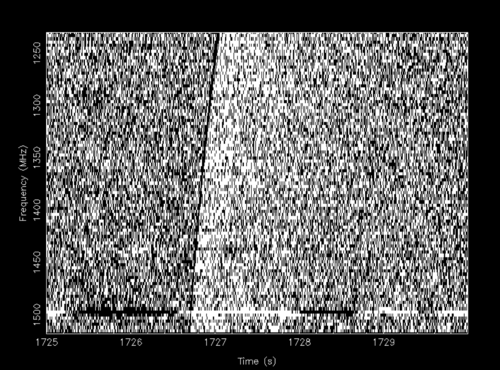
\includegraphics[width=0.8\textwidth]{figures/Lorimer Burst.png}
\caption{Ráfaga de Lorimer: observación de la primera ráfaga de radio rápida detectada, tal como la describió Lorimer en 2006.}
\label{fig:lorimer}
\end{figure}

\section{Problema}
Detectar FRBs en tiempo de procesamiento plantea desafíos considerables. Los radiotelescopios modernos generan volúmenes masivos de datos, lo que dificulta el procesamiento eficiente de observaciones en busca de eventos de milisegundos. A esto se suma la abundante interferencia de radiofrecuencia (RFI) de origen humano, que contamina las señales e imita pulsos astrofísicos, produciendo grandes listas de candidatos falsos. Los métodos tradicionales de búsqueda de pulsos individuales como los algoritmos implementados en suites clásicas tipo PRESTO y Heimdall se basan en dedispersión exhaustiva y umbrales fijos de detección, si bien han sido exitosos, son propensos a listas extensas de falsos positivos y requieren inspección manual intensiva, lo que limita su uso en operación en tiempo (casi) real \cite{Cordes_2003, Ransom_2003, Barsdell_2012}. Por otra parte, \textbf{DRAFTS} aporta modelos de detección y clasificación, pero no un pipeline operativo extremo a extremo.

\textbf{TODO (Problema específico)}: Completar con 3–4 frases que describan el vacío exacto en tu contexto (datos disponibles, limitaciones de herramientas actuales en tu entorno, necesidad de near-real-time, etc.).

\section{Objetivos}
\textbf{Objetivo general:} Diseñar e implementar un pipeline basado en DRAFTS para detección y clasificación de transientes de radio, y extenderlo a regímenes de alta frecuencia.\\
\textbf{Objetivos específicos:}
\begin{itemize}
  \item Integrar y operacionalizar los modelos de DRAFTS en un pipeline reproducible.
  \item Diseñar módulos de ingesta, preprocesado, detección, clasificación y reporte.
  \item Adaptar la búsqueda a frecuencias milimétricas (mm-wave) considerando sus particularidades.
  \item Evaluar desempeño (recall, precision, F1, latencia) en banda L y en mm-wave.
\end{itemize}

\textbf{TODO (Medición de objetivos)}: Indicar cómo verificarás cada objetivo (p.ej., latencia \(<\) N s/archivo de 32 GB; F1 \(>\) X en FRB121102).

\section{Preguntas de investigación e hipótesis}
¿Cómo se comporta la detección y clasificación de FRBs al comparar banda L con mm-wave? Hipótesis: la atenuación del patrón bow-tie en mm-wave disminuye sensibilidad de detectores basados en tiempo–DM, mitigable ampliando rango/step de DM y mediante validación por sub-bandas y clasificación a DM\(\approx 0\).

\textbf{TODO (Criterios de falsación)}: Expresar qué resultados refutarían/confirmarían la hipótesis (p.ej., recall relativo mm-wave/L-band, tasa de falsos DM\(\approx\)0).

\section{Principales contribuciones técnicas}
\begin{itemize}
  \item Pipeline DRAFTS-MB con módulos definidos, contratos I/O y configuración.
  \item Estrategias de chunking/slices/overlap con criterios formales de \(\Delta DM\) por smearing.
  \item Integración CenterNet (detección) + ResNet (clasificación) con umbrales robustos (MAD/IQR).
  \item Extensión y validación en mm-wave y lineamientos para operación near-real-time.
\end{itemize}

\textbf{TODO (Evidencias de contribución)}: Enumerar outputs verificables (scripts, configs, artefactos, figuras clave, IDs de commit).

\section{Alcance y limitaciones}
El trabajo se enfoca en búsqueda de pulsos individuales (single-pulse) y no aborda timing ni localización interferométrica plena. Se trabaja con PSRFITS/FIL, con disponibilidad de GPU estándar. Limitaciones incluyen RFI a DM\(\approx 0\), dependencia de metadatos fiables y variabilidad instrumental.

\textbf{TODO (Límites explícitos)}: Añadir supuestos concretos (p.ej., resolución temporal mínima, anchos de banda soportados, formatos exactos, versiones de librerías).

\section{Organización del documento}
Este documento se organiza en diez capítulos más anexos. El Capítulo 2 presenta el marco teórico; el 3, el estado del arte; el 4, los requisitos y el diseño del pipeline; el 5, la implementación; el 6, la metodología experimental y los datasets; el 7, los resultados en banda L; el 8, la extensión a mm-wave (ALMA); el 9, la discusión y amenazas a la validez; y el 10, las conclusiones y trabajo futuro.

\section{Posicionamiento frente a pipelines en tiempo real}
Como motivación y punto de comparación, se discuten arquitecturas operativas de CHIME/FRB, ASKAP/CRAFT y MeerTRAP, destacando diferencias en adquisición, backend, mitigación de RFI y criterios de decisión, que orientan los requisitos y decisiones del presente pipeline.

\newpage
\secnumbersection{DEFINICIÓN DEL PROBLEMA}

% Se debe definir el problema, es importante no confundir definir el problema con describir la solución. Por ejemplo: ``diseñar una arquitectura e implementar una plataforma ...'' es una solución, no un problema.
% 
% Algunos elementos que podrían ir en este capítulo son (no es necesario que vayan todos):
% \begin{itemize}
%     \item Breve descripción del contexto donde se realizará la memoria (organización, línea dentro de la Informática en la que se basa, etc.)
%     \item ¿Qué y cómo se realiza actualmente la situación que mejorarás con tu memoria?
%     \item ¿Qué actores o usuarios están involucrados?
%     \item ¿Qué dificultades tienen esos actores actualmente? ¿cuántos son? (ideal si se pueden poner estadísticas para así saber si existe un mercado razonable para la solución que propondrás en tu memoria, en el fondo saber cuántas personas u organizaciones tienen el mismo problema que estás definiendo)
%     \item ¿Qué podría pasar si en el corto o mediano plazo no se solucionan esas dificultades (¿es decir, si no se hiciera tu memoria, qué pasaría?; en el fondo justificar por qué conviene hacer tu memoria, ¿cuál es la motivación o interés de hacerla?).
%     \item ¿Qué competencia existe actualmente? (a lo mejor ya existe una solución al problema, pero por qué no sirve, o por qué tu solución sería mejor, también se puede enfocar a si este problema existe en otras realidades y cómo ha sido solucionado allí).
%     \item Precisar los objetivos y alcances de la memoria (o solución al problema).
% \end{itemize}
% 
% En este capítulo, de ser necesario puede usar referencias bibliográficas (velar porque sean recientes), una cita de ejemplo \cite{schwab2002cure} y otras más \cite{georget1994study,beaumont1990patient}.
% 
% Recuerde poner notas al pie de página que sean explicativas \footnote{Este es un ejemplo de una nota al pie de página. Puede indicar alguna URL, definiciones, aclarar alguna información pertinente del texto, citar algunas referencias, etc..}.
% 
% \subsection{SUBSECCIÓN DE PRUEBA}
% 
% Sed ut perspiciatis unde omnis iste natus error sit voluptatem accusantium doloremque laudantium, totam rem aperiam, eaque ipsa quae ab illo inventore veritatis et quasi architecto beatae vitae dicta sunt explicabo.
% 
% \subsubsection{SUBSUBSECCIÓN DE PRUEBA}
% 
% Nemo enim ipsam voluptatem quia voluptas sit aspernatur aut odit aut fugit, sed quia consequuntur magni dolores eos qui ratione voluptatem sequi nesciunt. Neque porro quisquam est, qui dolorem ipsum quia dolor sit amet.
% 
% \subsubsection{OTRA SUBSUBSECCIÓN DE PRUEBA}
% 
% Nemo enim ipsam voluptatem quia voluptas sit aspernatur aut odit aut fugit, sed quia consequuntur magni dolores eos qui ratione voluptatem sequi nesciunt. Neque porro quisquam est, qui dolorem ipsum quia dolor sit amet.
\subsection{Descripción}

Los \textit{Fast Radio Bursts} (FRBs) son  eventos transitorios  de milisegundos de origen extragaláctico. Su estudio se ha consolidado como una línea de investigación en radioastronomia y ciencia de datos, en la cual convergen desarrollos de instrumentación, procesamiento de señales y aprendizaje automático. En la actualidad, se han desarrollado métodos y modelos capaces de detectar y clasificar FRBs en distintos contextos, junto con marcos de trabajo que incorporan técnicas de aprendizaje profundo. Sin embargo, estas aproximaciones suelen estar limitadas a implementaciones específicas, de difícil reproducción y con escasa portabilidad. En particular, no se dispone de un flujo de procesamiento consolidado que pueda adaptarse a distintos entornos y extenderse a regímenes de alta frecuencia (mm-wave) sin necesidad de reentrenar los modelos. En este capítulo se describe los detalles de problema y se expone el enfoque que guiará el desarrollo de la memoria.


%Este capítulo formula el \textbf{problema} que aborda la memoria: la ausencia de un \textit{pipeline} operativo, reproducible y portable que permita \textbf{detectar y clasificar FRBs en tiempo (casi) real} y que, además, sea \textbf{extensible a regímenes de alta frecuencia} (mm-wave) sin reentrenar modelos. La investigación se sitúa en la intersección de la Informática (ingeniería de software y ML aplicado) y la radioastronomía, utilizando como base el marco conceptual y el código no finalizado de \textbf{DRAFTS}\footnote{\emph{Deep-learning Real-time pAstro nomy FRB TranSients} (DRAFTS). Se usa como punto de partida por disponer de modelos de detección y clasificación y de utilidades de procesamiento, pero su código requiere consolidación para uso productivo.}, sobre el cual se propone construir un \textit{pipeline} robusto.


%Esta limitación constituye el problema central de la memoria, que se aborda desde la intersección de la Informática —en particular la ingeniería de software y el aprendizaje automático— y la radioastronomía. Como punto de partida se emplea el marco conceptual y el código preliminar de DRAFTS\footnote{\emph{Deep-learning Real-time Astronomy FRB TranSients} (DRAFTS). Se utiliza como base inicial por contar con modelos de detección y clasificación y con utilidades de procesamiento, aunque su código requiere consolidación para uso productivo.}, sobre los cuales se plantea el diseño e implementación de un flujo de procesamiento más robusto, reproducible y portable.%

\medskip

Actualmente, la búsqueda de FRBs en radioastronomía se desarrolla principalmente en dos regímenes espectrales con características y desafíos distintos. En las frecuencias tradicionalmente utilizadas (bandas decimétricas, aproximadamente 300 MHz - 3 GHz), la detección se fundamenta en flujos de procesamiento clásicos que incluyen limpieza de interferencia de radiofrecuencia (RFI), dedispersión mediante rejillas de medida de dispersión (DM), filtrado por \emph{matched filtering}, y la posterior generación y depuración de candidatos. A pesar de la madurez relativa de estos métodos, la etapa de depuración continúa demandando curaduría manual extensiva y el desarrollo de scripts \emph{ad hoc} específicos para cada equipo de investigación.


En contraste, el régimen de alta frecuencia (30--100 GHz, ondas milimétricas), particularmente en configuraciones de arreglo en fase (\emph{phased array}) como las implementadas en ALMA\footnote{La configuración de \emph{phased array} permite la formación de un haz coherente y el registro de series temporales de alta resolución temporal, elementos esenciales para experimentos de detección de transientes y pulsos.}, presenta una ventana científica prometedora pero carece de \textit{pipelines} estandarizados. En estas frecuencias, el retardo dispersivo $\Delta t\propto \mathrm{DM},\nu^{-2}$ es menor, los patrones diagnósticos (\emph{bow-tie} en tiempo--DM) se atenúan, y los desarrollos actuales permanecen en estado de prototipo.

%Hoy, la búsqueda de FRBs en bandas decimétricas se apoya en flujos clásicos (limpieza RFI, dedispersión en rejillas de DM, filtrado por \emph{matched filtering}, generación y depuración de candidatos). La depuración sigue demandando curaduría manual y scripts ad hoc por equipo. En \textbf{alta frecuencia} (30--100,GHz; modo \emph{phased} en arreglos como ALMA\footnote{\emph{Phased array} permite formar un haz coherente y registrar series temporales de alta resolución para experimentos de transientes/pulsos.}), la ventana científica es prometedora pero \textbf{no existen \textit{pipelines} estandarizados y de propósito general} para transientes de milisegundos: los datos son distintos (menor retardo dispersivo observable, otras sistemáticas) y los desarrollos actuales son prototipos.%

\medskip

En vista de estos desafíos técnicos diferenciados, se han desarrollado herramientas clásicas como PRESTO y Heimdall, eficaces en bandas L y S pero limitadas para escenarios de alta frecuencia. En aprendizaje profundo, marcos como \textbf{DRAFTS} han explorado aproximaciones prometedoras mediante detección en mapas tiempo--DM y clasificación binaria sobre \emph{patches} tiempo--frecuencia. Sin embargo, la transición hacia un \textit{pipeline} operativo que incorpore principios sólidos de ingeniería de software y sea extensible entre regímenes frecuenciales permanece como una brecha crítica.

Los desafíos operativos comunes a ambos regímenes incluyen: fricción computacional (archivos grandes y procesamiento intensivo que genera latencia crítica para alertas de seguimiento), altas tasas de falsos positivos (RFI y artefactos instrumentales que exigen validación manual), y la ausencia de pipelines end-to-end que integren modelos de aprendizaje automático con ingeniería de datos, métricas y reportabilidad robustas.

\begin{table}[h]
\centering
\caption{\textbf{Comparación de características técnicas entre regímenes espectrales relevantes para el diseño del pipeline.}}
\vspace{0.5em}
\begin{tabular}{|l|l|l|}
\toprule
\textbf{Aspecto} & \textbf{0.3--3\,GHz} & \textbf{30--100\,GHz} \\
\midrule
Retardo por dispersión & Alto; patrones claros en tiempo--DM & Bajo; patrones atenuados \\
RFI/sistemáticas & RFI ancha banda & Atmósfera, estabilidad de fase, distinta RFI \\
Productos útiles & Waterfalls, tiempo--DM & Tiempo--frecuencia, polarización/diagnósticos alternativos \\
Disponibilidad de software & Pipelines consolidados & Prototipos, sin estándar general \\
\bottomrule
\vspace{0.2em}
\end{tabular}
\raggedright
\small{\textit{Nota: RFI = Radio Frequency Interference (Interferencia de Radiofrecuencia); DM = Dispersion Measure (Medida de Dispersión).}}
\end{table}

\medskip
%Hoy por hoy existen herramientas clásicas (PRESTO/Heimdall) y marcos específicos de proyectos que han sido eficaces en L/S-band, pero su adopción como \textbf{producto} general es limitada, pues no se consideran escenarios de alta frecuencia. En DL, \textbf{DRAFTS} sugiere una vía: detección en mapas tiempo--DM (estimación de $(t_{arr},,\mathrm{DM})$) + \emph{patch} tiempo--frecuencia para clasificación binaria. La brecha es llevar ese enfoque a un \textit{pipeline} reproducible, con ingeniería de software, monitoreo, métricas y \textbf{adaptación a alta frecuencia} sin reentrenar modelos.



\medskip
%Entonces, luego del contexto anterior, presentamos la formulación del problema; dado un flujo de datos de radioastronomía (FITS/PSRFITS u otros formatos) y dos modelos preentrenados (detección y clasificación), se requiere construir un \textbf{pipeline operativo, reproducible y portable} que: (i) procese en lotes y en línea con control de recursos, (ii) reduzca falsos positivos con una segunda criba basada en DL, (iii) produzca salidas auditables (catálogo de candidatos, recortes, figuras, métricas), y (iv) \textbf{funcione en alta frecuencia} parametrizando adecuadamente DM-grids, escalas temporales y productos diagnósticos (incluida polarización cuando esté disponible). Todo ello \textbf{sin reentrenar} los modelos base.%

Considerando este contexto, el presente trabajo aborda la siguiente formulación del problema: dado un flujo de datos de radioastronomía (FITS/PSRFITS u otros formatos) y dos modelos preentrenados (detección y clasificación), se requiere construir un **pipeline operativo, reproducible y portable** que: (i) procese datos en lotes y en línea con control eficiente de recursos, (ii) reduzca falsos positivos mediante una segunda criba basada en aprendizaje profundo, (iii) genere salidas completamente auditables (catálogo de candidatos, recortes, figuras diagnósticas y métricas de rendimiento), y (iv) **sea extensible a regímenes de alta frecuencia** mediante parametrización adecuada de rejillas DM, escalas temporales y productos diagnósticos (incluida polarización cuando esté disponible). Todo ello **sin requerir 

\medskip
%La propuesta ataca un cuello de botella real (latencia + robustez) y agrega valor transversal (portabilidad y estandarización). El impacto esperado es doble: (i) \emph{operativo}, al disminuir fricción y tiempos de análisis; (ii) \emph{científico}, al habilitar búsquedas consistentes en mm-wave y facilitar comparabilidad entre campañas.%

Esta propuesta aborda limitaciones críticas en el área: la alta latencia computacional que impide alertas oportunas de seguimiento, y la falta de robustez operativa que requiere intervención manual extensiva para validar candidatos. La solución aporta valor transversal mediante portabilidad y estandarización de procesos. El impacto esperado es doble: (i) **operativo**, al reducir significativamente los tiempos de procesamiento y automatizar la validación de candidatos; y (ii) **científico**, al habilitar búsquedas sistemáticas y consistentes en el régimen de ondas milimétricas y facilitar la comparabilidad entre diferentes campañas observacionales.

\medskip

\subsection{Objetivos y Resultados Esperados}

\textbf{Objetivos}
\begin{itemize}
\item \textbf{General:} Desarrollar un \textbf{pipeline astronómico operativo} para \textbf{detección y clasificación de FRBs} basado en dos CNN preentrenadas, \textbf{extensible a regímenes de alta frecuencia} sin reentrenamiento.
\item \textbf{Específicos:}
\begin{enumerate}
\item Integrar los modelos de \emph{detección} y \emph{clasificación} en un flujo robusto y reproducible: ingesta $\to$ preprocesamiento $\to$ inferencia $\to$ posprocesamiento $\to$ reporte auditable.
\item Implementar optimizaciones de rendimiento: procesamiento eficiente de archivos grandes, gestión de memoria, aceleración computacional y registro completo de operaciones.
\item Parametrizar el flujo para \textbf{adaptación a alta frecuencia} (rejillas DM, ventanas temporales, productos Stokes/polarización) \textbf{sin reentrenamiento} de modelos.
\item Validar el sistema sobre datos previamente analizados, \textbf{igualando o superando} recuentos reportados y caracterizando latencia, \emph{precision} y \emph{recall}.
\item Implementar productos diagnósticos específicos para ondas milimétricas y realizar análisis exploratorios para caracterizar las propiedades distintivas de FRBs en alta frecuencia.
\end{enumerate}
\end{itemize}

\medskip
En esta memoria, no se contempla reentrenar modelos ni desarrollar \emph{backends} instrumentales; el foco es \textbf{inferencias y orquestación} a partir de modelos existentes y datos crudos/reducidos.

\medskip
\noindent\textbf{Resultados esperados}
\begin{itemize}
\item \emph{Pipeline} end-to-end ejecutable por línea de comandos y/o servicio, con documentación completa y suite de pruebas automatizadas.
\item Reporte comparativo de desempeño que incluya métricas de \emph{recall}, \emph{precision}, \emph{throughput} y latencia por GB/archivo procesado.
\item Conjunto de figuras y \emph{notebooks} ilustrativos que demuestren la aplicación del pipeline en el régimen de ondas milimétricas.
\end{itemize}

\begin{figure}[h]
\centering
% \includegraphics[width=0.9\textwidth]{workflow_propuesto.pdf}
\caption{\textbf{Sugerencia de figura:} Flujo actual (dedispersión + candidatos + curaduría) versus flujo propuesto (detección DL + clasificación DL + reporte). Señalar puntos de latencia y reducción de falsos positivos.}
\end{figure}

\newpage
\newpage
\secnumbersection{MARCO TEÓRICO}

\section{FRBs y pulsos individuales: DM, dispersión, ancho y S/N}
Las FRBs son pulsos de duración típica de milisegundos, caracterizados por su \textit{Medida de Dispersión} (DM), ancho intrínseco/observado y relación señal/ruido (S/N). La dispersión en el medio ionizado introduce un retardo en frecuencia que se aproxima por
\[\Delta t\,\,\mathrm{[ms]} \approx 4.15\times10^3\,\mathrm{DM}\,\left(\nu_1^{-2}-\nu_2^{-2}\right),\]
donde \(\nu\) se expresa en MHz. El ensanchamiento por dispersión y efectos instrumentales (\textit{smearing}) limita la sensibilidad si excede el ancho del pulso.

\section{Plano tiempo--DM y patrón ``bow-tie''}
La búsqueda de pulsos individuales se realiza en el plano tiempo--DM, donde una ráfaga astrofísica genera un patrón en ``corbatín'' (\textit{bow-tie}). La apertura del patrón depende de la cobertura en frecuencia y de la DM del evento; el máximo S/N aparece cerca de la DM verdadera.

\section{RFI: criterios de discriminación astrofísico vs terrestre}
La RFI suele concentrarse en bandas estrechas, presenta DM cercana a cero y carece de la dispersión cromática propia de señales cósmicas. Criterios como consistencia en sub-bandas, simetría temporal, estabilidad de DM y persistencia espacial ayudan a discriminar eventos astrofísicos.

\section{Dedispersión y waterfalls (sin y con dedispersión)}
Los \textit{waterfalls} crudos muestran la dispersión en frecuencia; tras dedispersar a una DM candidata, un pulso real se alinea temporalmente a través de canales. La inspección conjunta tiempo--DM y \textit{waterfalls} dedispersados es clave para validar candidatos.

\section{Particularidades a alta frecuencia (mm-wave)}
A frecuencias milimétricas el retardo por dispersión es menor, atenuando el ``bow-tie'' y reduciendo la ganancia de S/N asociada a la dedispersión. Esto exige ampliar el rango y el paso de DM o estrategias de validación por sub-bandas y clasificación complementaria.

\section{Telescopios y datos relevantes}
Se consideran instrumentos y formatos representativos: FAST y Effelsberg (banda L), y ALMA en modo \textit{phased} para frecuencias milimétricas. Formatos habituales: PSRFITS/SEARCH y \texttt{FIL}, con metadatos esenciales como \texttt{TBIN}, \texttt{NCHAN}, ancho de banda, frecuencias y tiempos de inicio en MJD.

\section{Convenciones de polarización (PSR/IEEE) y PSRFITS/PSRCHIVE}
Se adopta la convención PSR/IEEE para Stokes \(I,Q,U,V\). La correcta interpretación y almacenamiento de polarización en PSRFITS y su tratamiento en PSRCHIVE son relevantes para análisis avanzados y mitigación de RFI.

\section{Trazabilidad temporal}
Se resguarda trazabilidad mediante sellos de tiempo absolutos (MJD topocéntrico) y consistencia con modelos temporales (p.ej., TEMPO2), asegurando coherencia entre bloques y reproductibilidad de ventanas temporales.

\newpage
\secnumbersection{PROPUESTA DE SOLUCIÓN}

Se debe desarrollar la solución propuesta. Los subcapítulos por poner aquí son propios del autor. Se sugiere mencionar metodología usada. Es conveniente incorporar figuras y tablas para aclarar la solución, que deben indicar el número de la figura, su nombre y su autor o fuente (si las diseñas tú, la fuente es ``Elaboración propia''). Ver ejemplos en esta página y en la siguiente.

Cabe mencionar que aquí está la esencia del trabajo en lo que se refiere al aporte creativo del memorista, es el momento de demostrar que usted es un destacado profesional que creó, diseñó y/o llevó a cabo la solución propuesta.

\subsection{EJEMPLO DE COMO CITAR FIGURAS E ILUSTRACIONES}

Se colocó una imagen que se puede referenciar también desde el texto (Ver figura \ref{fig:malla}).

\begin{figure}[h]
\centering
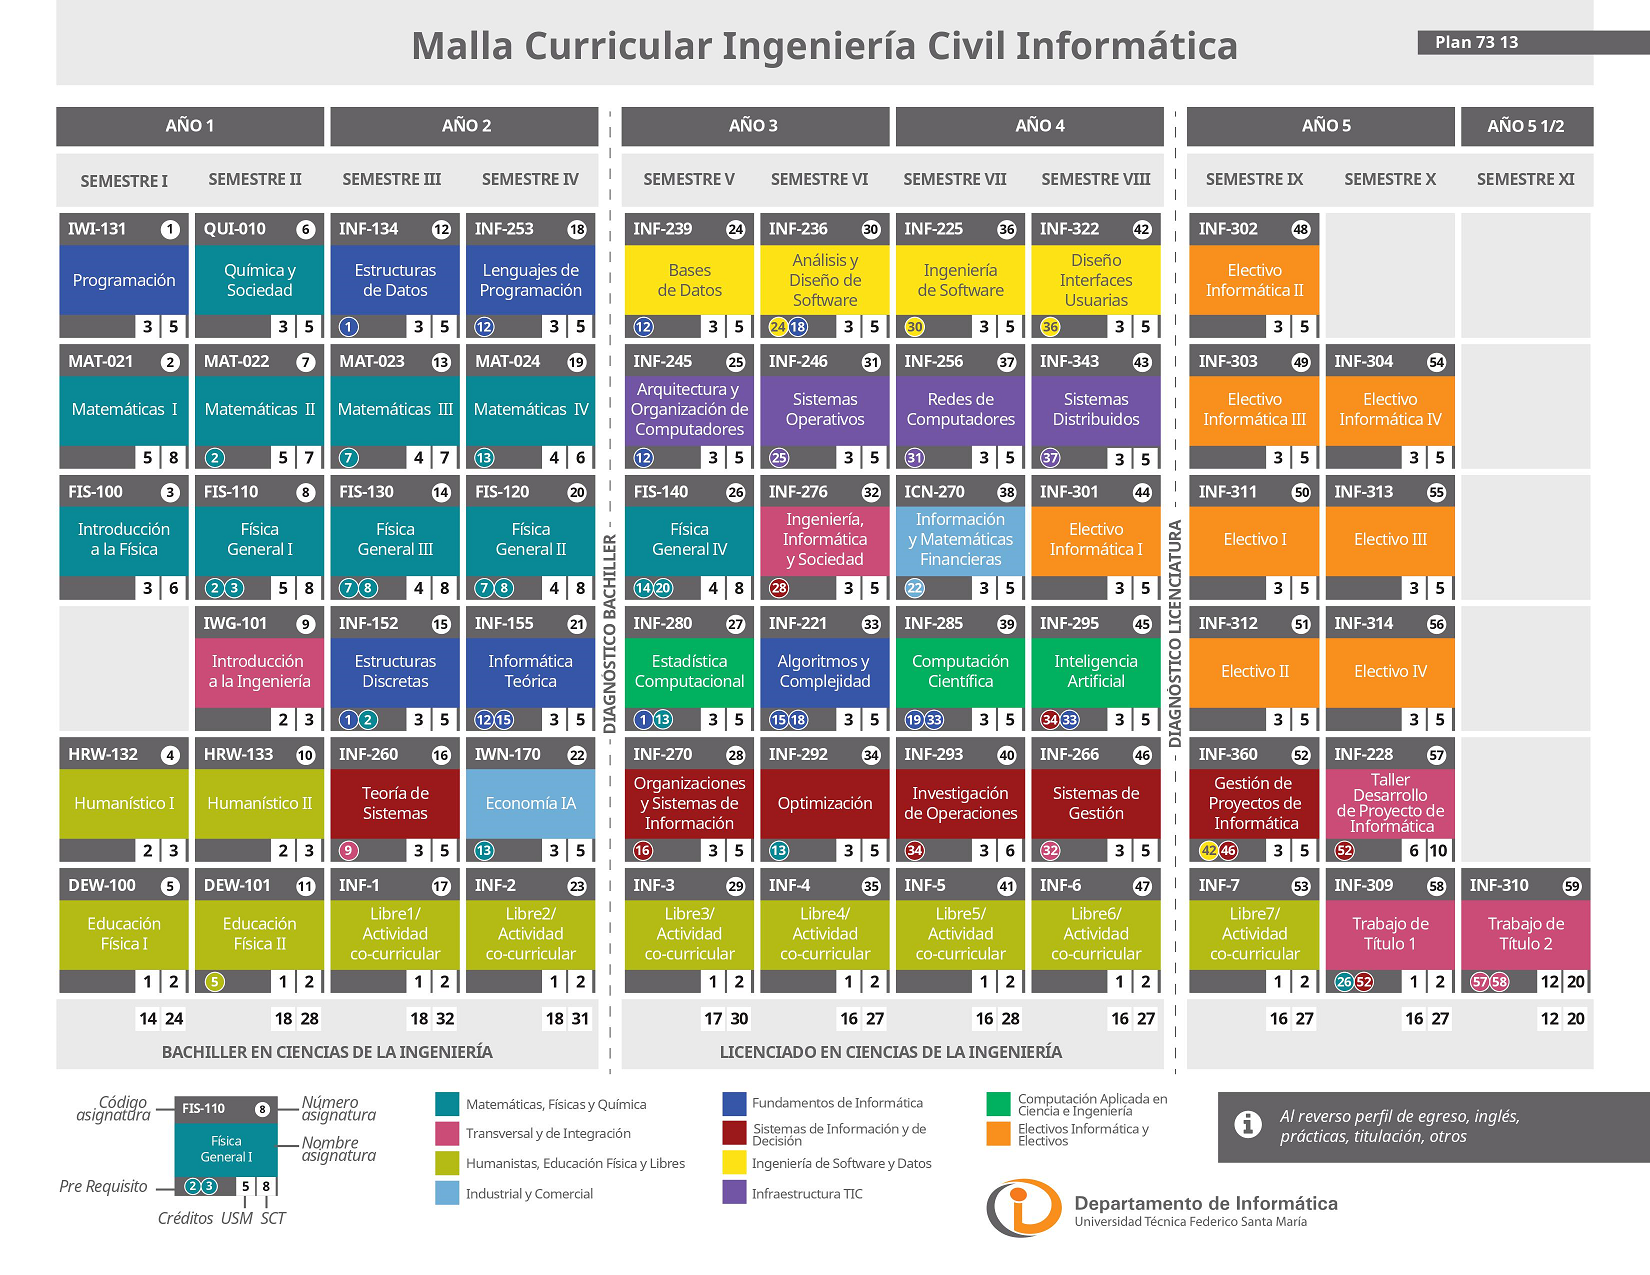
\includegraphics[width=0.8\textwidth]{malla_ingenieria_informatica}
\caption{\label{fig:malla} Malla Curricular Ingeniería Civil Informática.} Fuente: Departamento de Informática.
\end{figure}



\newpage
\secnumbersection{VALIDACIÓN DE LA SOLUCIÓN}

Se debe validar la solución propuesta. Esto significa probar o demostrar que la solución propuesta es válida para el entorno donde fue planteada.

Tradicionalmente es una etapa crítica, pues debe comprobarse por algún medio que vuestra propuesta es básicamente válida. En el caso de un desarrollo de software es la construcción y sus pruebas; en el caso de propuestas de modelos, guías o metodologías podrían ser desde la aplicación a un caso real hasta encuestas o entrevistas con especialistas; en el caso de mejoras de procesos u optimizaciones, podría ser comparar la situación actual (previa a la memoria) con la situación final (cuando la memoria está ya implementada) en base a un conjunto cuantitativo de indicadores o criterios.

\subsection{EJEMPLO DE COMO CITAR TABLAS}

Se colocó una tabla que se puede referenciar también desde el texto (Ver tabla \ref{table:coloquios}).

\begin{table}[h]
    \centering
    \caption{\label{table:coloquios} Coloquios del Ciclo de Charlas Informática.} Fuente: Elaboración Propia.
    \begin{tabular}{|p{7cm}|p{7cm}|}
        \hline
        Título Coloquio & Presentador, País \\
        \hline
        ``Sensible, invisible, sometimes tolerant, heterogeneous, decentralized and interoperable... and we still need to assure its quality...''' & Guilherme Horta Travassos, Brasil.\\
        \hline
        ``Dispersed Multiphase Flow Modeling: From Environmental to Industrial Applications''' & Orlando Ayala, EE.UU.\\
        \hline
        ``Líneas de Producto Software Dinámicas para Sistemas atentos el Contexto''' & Rafael Capilla, España.\\
        \hline
        ... & ... \\
        \hline
    \end{tabular}
\end{table}

\newpage
\secnumbersection{CONCLUSIONES Y TRABAJO FUTURO}

\subsection{Resumen de aportes y respuestas a las preguntas}
Se sintetizan las contribuciones técnicas del pipeline DRAFTS-MB, su desempeño en banda L y su extensión a frecuencias milimétricas, respondiendo las preguntas de investigación sobre sensibilidad y precisión comparativas.

\subsection{Lecciones aprendidas de llevar DRAFTS a producción}
Se discuten hallazgos sobre integración de modelos, control del \textit{trials factor}, robustez a RFI y gestión de memoria/latencia en operación \textit{near-real-time}.

\subsection{Próximos pasos}
Se delinean reentrenos específicos para mm-wave, adaptación de dominio, procesamiento en flujo continuo (streaming) e integración con pipelines de observatorios.

\textbf{TODO}: Priorizar 3 acciones con plazos tentativos (p.ej., reentrenos mm-wave, pruebas en Band 3, integración con backend).

\subsection{Líneas de trabajo futuro}
Se proponen líneas para localización y consistencia por sub-bandas, validaciones cruzadas con pipelines externos (CHIME/FRB, MeerTRAP, ASKAP/CRAFT), y estrategias FAIR para datos/modelos. Si la detección falla en mm-wave por falta de \textit{bow-tie} (línea casi recta en tiempo--DM), reentrenar/adaptar el modelo o desarrollar uno nuevo específico para regímenes milimétricos con \textit{plots} característicos.


\newpage
\secnumberlesssection{ANEXOS}

En los Anexos se incluye todo aquel material complementario que no es parte del contenido de los capítulos de la memoria, pero que permiten a un lector contar con un contenido adjunto relacionado con el tema.

\subsection{ANEXO A: RESULTADOS DE VALIDACIÓN - BAJAS FRECUENCIAS (FRB 121102)}

\subsubsection{Bursts Confirmados por Literatura}

\begin{table}[H]
    \centering
    \caption{Bursts de FRB121102 confirmados por literatura (detectados por DRAFTS++ y reportados por Cruces et al. 2020). \textit{Fuente: Elaboración propia basada en Cruces et al. (2020) \cite{cruces2020frb121102}.}}
    \label{tab:anexo_confirmed_bursts}
    \begin{tabular}{|c|c|c|c|c|c|c|c|}
        \hline
        \multicolumn{4}{|c|}{\textbf{Columna 1}} & \multicolumn{4}{|c|}{\textbf{Columna 2}} \\
        \hline
        \textbf{File} & \textbf{DM} & \textbf{Time(s)} & \textbf{MJD} & \textbf{File} & \textbf{DM} & \textbf{Time(s)} & \textbf{MJD} \\
        \hline
        3096 & 564.15 & 114.059783 & 58440.83884126 & 3100 & 565.97 & 1253.032154 & 58441.01915005 \\
        3096 & 564.64 & 2172.299182 & 58440.86266456 & 3100 & 564.96 & 2090.123919 & 58441.02883908 \\
        3098 & 564.77 & 229.680524 & 58440.92373659 & 3100 & 557.7 & 2090.126104 & 58441.02883929 \\
        3098 & 565.35 & 1359.279991 & 58440.93681124 & 3100 & 563.53 & 2172.314365 & 58441.02979044 \\
        3098 & 563.5 & 3445.629 & 58440.96095990 & 3101 & 558.49 & 1160.627268 & 58441.05983026 \\
        3099 & 557.55 & 2331.324798 & 58440.98983520 & 3101 & 557.92 & 1174.354439 & 58441.05998916 \\
        3099 & 564.17 & 3111.182227 & 58440.99886157 & 3101 & 558.01 & 1297.028219 & 58441.06140906 \\
        3100 & 565.38 & 254.527406 & 58441.00759278 & 3101 & 566.12 & 1571.448422 & 58441.06458515 \\
        3100 & 557.11 & 310.032903 & 58441.00823545 & 3101 & 565.31 & 1814.433191 & 58441.06739762 \\
        3100 & 563.91 & 686.839999 & 58441.01259666 & 3102 & 563.14 & 1571.362789 & 58441.10636851 \\
        3100 & 564.75 & 942.375786 & 58441.01555436 & 3102 & 556.67 & 1823.937659 & 58441.10929213 \\
        3100 & 563.87 & 1148.701027 & 58441.01794252 & 3102 & 563.94 & 2099.014533 & 58441.11247584 \\
        \hline
    \end{tabular}
\end{table}

\subsubsection{Nuevos Candidatos Sin Confirmar}

\begin{table}[H]
    \centering
    \caption{Nuevos candidatos a bursts detectados únicamente por DRAFTS++ (pendientes de confirmación científica). \textit{Fuente: Elaboración propia}.}
    \label{tab:anexo_candidate_bursts}
    \begin{tabular}{|c|c|c|c|c|c|c|c|}
        \hline
        \multicolumn{4}{|c|}{\textbf{Columna 1}} & \multicolumn{4}{|c|}{\textbf{Columna 2}} \\
        \hline
        \textbf{File} & \textbf{DM} & \textbf{Time(s)} & \textbf{MJD} & \textbf{File} & \textbf{DM} & \textbf{Time(s)} & \textbf{MJD} \\
        \hline
        3096 & 579.6 & 1208.742 & 58440.851511757 & 3100 & 260.22 & 3037.433692 & 58441.03980380 \\
        3096 & 565.46 & 2789.205716 & 58440.86980499 & 3101 & 380.95 & 841.313157 & 58441.05613900 \\
        3096 & 484.19 & 3475.569268 & 58440.87775151 & 3101 & 555.9 & 2973.492401 & 58441.08081351 \\
        3098 & 581.24 & 2745.689702 & 58440.93681364 & 3102 & 564.79 & 841.23932 & 58441.09791759 \\
        3098 & 571.6 & 3179.596 & 58440.95285796 & 3102 & 565.27 & 3179.698804 & 58441.12498428 \\
        3099 & 411.4 & 480.104 & 58440.96840787 & & & & \\
        3099 & 420.31 & 2491.019865 & 58440.99168722 & & & & \\
        3099 & 396.29 & 3205.235999 & 58440.99995461 & & & & \\
        3100 & 404.21 & 2638.652812 & 58441.03519230 & & & & \\
        \hline
    \end{tabular}
\end{table}

\subsubsection{Nuevos Eventos Confirmados}

\begin{table}[H]
    \centering
    \caption{Nuevos eventos de bursts 100\% confirmados por el grupo de astrónomos colaboradores. \textit{Fuente: Elaboración propia}.}
    \label{tab:anexo_new_confirmed_bursts}
    \begin{tabular}{|c|c|c|c|}
        \hline
        \textbf{File} & \textbf{DM} & \textbf{Time(s)} & \textbf{MJD} \\
        \hline
        3096 & 563.6 & 2421.559296 & 58440.86554968 \\
        3102 & 564.88 & 723.455399 & 58441.09655428 \\
        \hline
    \end{tabular}
\end{table}

\subsection{ANEXO B: RESULTADOS DE VALIDACIÓN - ALTAS FRECUENCIAS (ALMA)}

\subsubsection{Pulsos Confirmados por Literatura y Colaboradores}

\begin{table}[H]
    \centering
    \caption{Pulsos del magnetar PSR J1745-2900 confirmados por el pipeline de SNR + clasificación binaria. \textit{Fuente: Elaboración propia}.}
    \label{tab:anexo_alma_confirmed_pulses}
    \begin{tabular}{|c|c|c|c|}
        \hline
        \multicolumn{2}{|c|}{\textbf{Columna 1}} & \multicolumn{2}{|c|}{\textbf{Columna 2}} \\
        \hline
        \textbf{File} & \textbf{Time(s)} & \textbf{File} & \textbf{Time(s)} \\
        \hline
        134 & 47.13472 & 152\_0006 & 24.889344 \\
        134 & 43.136 & 152\_0007 & 10.110976 \\
        142\_0002 & 17.076224 & 220\_0005 & 33.619968 \\
        142\_0002 & 43.450368 & 227\_0002 & 14.961664 \\
        142\_0002 & 47.204352 & 227\_0003 & 15.294464 \\
        142\_0008 & 45.2608 & 227\_0003 & 22.811648 \\
        142\_0008 & 0.94208 & 227\_0005 & 8.370176 \\
        142\_0008 & 12.06784 & 227\_0005 & 46.034944 \\
        143\_0005 & 35.405824 & 227\_0007 & 8.93952 \\
        143\_0005 & 43.011072 & 227\_0008 & 5.497856 \\
        143\_0006 & 5.682176 & 227\_0008 & 31.889408 \\
        143\_0006 & 43.312128 & 230\_0001 & 32.161792 \\
        143\_0007 & 13.481984 & 230\_0004 & 40.580096 \\
        152\_0004 & 16.733184 & 240\_0003 & 10.92608 \\
        152\_0005 & 16.872448 & 240\_0003 & 41.061376 \\
        152\_0006 & 17.347584 & 240\_0004 & 33.820672 \\
        240\_0004 & 41.295872 & 242\_0002 & 2.686976 \\
        242\_0003 & 10.527744 & 242\_0004 & 6.90176 \\
        242\_0004 & 44.729344 & 242\_0004 & 48.4864 \\
        142\_0003 & 36.188 & 142\_0006 & 3.180 \\
        142\_0006 & 18.291 & 230\_0002 & 28.686 \\
        242\_0005 & 26.167 & & \\
        \hline
    \end{tabular}
\end{table}

\subsubsection{Candidatos Detectados Sin Validar}

\begin{table}[H]
    \centering
    \caption{Muestra de candidatos a pulsos detectados por el pipeline de SNR + clasificación binaria (pendientes de validación científica). \textit{Fuente: Elaboración propia}.}
    \label{tab:anexo_alma_candidate_pulses}
    \begin{tabular}{|c|c|c|c|c|c|c|c|}
        \hline
        \multicolumn{2}{|c|}{\textbf{Columna 1}} & \multicolumn{2}{|c|}{\textbf{Columna 2}} & \multicolumn{2}{|c|}{\textbf{Columna 3}} & \multicolumn{2}{|c|}{\textbf{Columna 4}} \\
        \hline
        \textbf{File} & \textbf{Time(s)} & \textbf{File} & \textbf{Time(s)} & \textbf{File} & \textbf{Time(s)} & \textbf{File} & \textbf{Time(s)} \\
        \hline
        134 & 19.321856 & 142\_0002 & 32.121856 & 143\_0005 & 28.07296 & 152\_0004 & 5.436416 \\
        134 & 42.656768 & 142\_0002 & 32.157696 & 143\_0005 & 27.943936 & 152\_0004 & 43.129856 \\
        134 & 27.789312 & 142\_0002 & 39.4496 & 143\_0005 & 28.066816 & 152\_0004 & 43.204608 \\
        134 & 27.79648 & 142\_0002 & 39.379968 & 143\_0005 & 28.0832 & 152\_0005 & 5.716992 \\
        134 & 28.04224 & 142\_0002 & 39.441408 & 143\_0005 & 31.215616 & 152\_0005 & 5.712896 \\
        134 & 35.597312 & 142\_0002 & 47.19104 & 143\_0005 & 35.395584 & 152\_0005 & 32.200704 \\
        134 & 35.707904 & 142\_0002 & 47.213568 & 143\_0005 & 42.998784 & 152\_0005 & 32.114688 \\
        134 & 35.699712 & 142\_0002 & 50.910208 & 143\_0005 & 43.019264 & 152\_0005 & 35.866624 \\
        134 & 43.13088 & 142\_0002 & 50.850816 & 143\_0005 & 51.380224 & 152\_0006 & 0.086016 \\
        134 & 43.118592 & 142\_0008 & 3.85024 & 143\_0006 & 1.68448 & 152\_0006 & 13.304832 \\
        134 & 50.5088 & 142\_0008 & 3.847168 & 143\_0006 & 1.869824 & 152\_0006 & 13.309952 \\
        142\_0002 & 9.66144 & 142\_0008 & 3.95264 & 143\_0006 & 1.864704 & 152\_0006 & 17.335296 \\
        142\_0002 & 13.113344 & 142\_0008 & 3.960832 & 143\_0006 & 5.676032 & 152\_0006 & 17.355776 \\
        142\_0002 & 13.324288 & 142\_0008 & 14.973952 & 143\_0006 & 5.694464 & 152\_0006 & 24.886272 \\
        142\_0002 & 13.27104 & 142\_0008 & 33.987584 & 143\_0006 & 5.758976 & 152\_0007 & 10.145792 \\
        142\_0002 & 17.057792 & 142\_0008 & 45.253632 & 143\_0006 & 5.751808 & 152\_0007 & 33.952768 \\
        142\_0002 & 28.486656 & 142\_0008 & 46.698496 & 143\_0006 & 9.422848 & 152\_0007 & 47.827968 \\
        142\_0002 & 28.484608 & 143\_0003 & 0.953344 & 143\_0006 & 9.41056 & 152\_0007 & 47.816704 \\
        142\_0002 & 31.926272 & 143\_0003 & 0.961536 & 143\_0006 & 9.509888 & 152\_0007 & 47.837184 \\
        142\_0002 & 32.141312 & 143\_0003 & 12.058624 & 143\_0006 & 16.976896 & 220\_0005 & 33.608704 \\
        220\_0005 & 33.630208 & 220\_0006 & 3.919872 & 220\_0006 & 3.917824 & 220\_0006 & 10.624 \\
        227\_0002 & 11.006976 & 227\_0002 & 10.95168 & 227\_0002 & 10.99264 & 227\_0002 & 11.014144 \\
        227\_0002 & 11.039744 & 227\_0002 & 11.060224 & 227\_0002 & 11.094016 & 227\_0002 & 11.247616 \\
        227\_0002 & 11.104256 & 227\_0002 & 11.184128 & 227\_0002 & 11.239424 & 227\_0002 & 11.25888 \\
        227\_0002 & 11.322368 & 227\_0002 & 14.650368 & 227\_0002 & 14.874624 & 227\_0002 & 14.949376 \\
        227\_0002 & 18.761728 & 227\_0002 & 33.583104 & 227\_0002 & 33.813504 & 227\_0002 & 48.873472 \\
        227\_0002 & 48.861184 & 227\_0002 & 48.878592 & 227\_0003 & 4.013056 & 227\_0003 & 4.009984 \\
        227\_0003 & 11.630592 & 227\_0003 & 11.624448 & 227\_0003 & 12.691456 & 227\_0003 & 12.689408 \\
        227\_0003 & 32.550912 & 227\_0005 & 8.363008 & 227\_0005 & 8.491008 & 227\_0005 & 38.595584 \\
        227\_0005 & 42.27584 & 227\_0005 & 46.02368 & 227\_0005 & 49.50528 & 227\_0005 & 8.778752 \\
        227\_0007 & 8.9856 & 227\_0007 & 16.310272 & 227\_0007 & 31.483904 & 227\_0007 & 38.116352 \\
        227\_0007 & 38.905856 & 227\_0007 & 39.131136 & 227\_0007 & 42.71616 & 227\_0007 & 42.872832 \\
        227\_0008 & 5.382144 & 227\_0008 & 5.485568 & 227\_0008 & 5.502976 & 227\_0008 & 8.895488 \\
        227\_0008 & 11.184128 & 227\_0008 & 11.18208 & 227\_0008 & 12.75904 & 227\_0008 & 12.75392 \\
        227\_0008 & 12.875776 & 227\_0008 & 43.020288 & 227\_0008 & 43.01312 & 227\_0008 & 43.18208 \\
        227\_0008 & 43.174912 & 227\_0008 & 43.199488 & 227\_0008 & 46.768128 & 227\_0008 & 46.763008 \\
        230\_0001 & 36.09088 & 230\_0001 & 43.457536 & 230\_0001 & 43.467776 & 230\_0001 & 43.459584 \\
        230\_0001 & 51.01568 & 230\_0001 & 51.011584 & 230\_0001 & 51.03104 & 230\_0001 & 51.106816 \\
        230\_0004 & 2.967552 & 230\_0004 & 2.936832 & 230\_0004 & 6.675456 & 230\_0004 & 6.665216 \\
        230\_0004 & 18.024448 & 230\_0004 & 18.016256 & 230\_0004 & 21.552128 & 230\_0004 & 25.658368 \\
        230\_0004 & 25.655296 & 230\_0004 & 29.430784 & 230\_0004 & 40.567808 & 230\_0004 & 40.589312 \\
        230\_0004 & 40.715264 & 230\_0004 & 44.304384 & 230\_0004 & 44.391424 & 230\_0004 & 44.387328 \\
        230\_0004 & 47.875072 & 230\_0004 & 48.137216 & 230\_0004 & 47.990784 & 230\_0004 & 48.130048 \\
        240\_0003 & 14.578688 & 240\_0003 & 14.57664 & 240\_0003 & 14.825472 & 240\_0003 & 29.700096 \\
        240\_0003 & 29.800448 & 240\_0003 & 40.748032 & 240\_0003 & 40.738816 & 240\_0003 & 41.051136 \\
        240\_0003 & 41.073664 & 240\_0003 & 41.071616 & 240\_0003 & 48.601088 & 240\_0003 & 48.591872 \\
        240\_0003 & 49.815552 & 240\_0004 & 3.662848 & 240\_0004 & 9.182208 & 240\_0004 & 15.062016 \\
        240\_0004 & 15.059968 & 240\_0004 & 22.561792 & 240\_0004 & 22.516736 & 240\_0004 & 33.550336 \\
        240\_0004 & 33.568768 & 240\_0004 & 33.586176 & 240\_0004 & 41.07264 & 240\_0004 & 41.284608 \\
        240\_0004 & 44.942336 & 240\_0004 & 45.095936 & 240\_0004 & 45.088768 & 242\_0002 & 25.27744 \\
        242\_0002 & 25.271296 & 242\_0002 & 31.647744 & 242\_0002 & 37.50912 & 242\_0002 & 37.753856 \\
        242\_0002 & 51.538944 & 242\_0003 & 21.809152 & 242\_0003 & 21.881856 & 242\_0003 & 29.3632 \\
        242\_0003 & 36.992 & 242\_0003 & 36.985856 & 242\_0003 & 37.00224 & 242\_0003 & 40.650752 \\
        242\_0003 & 40.64768 & 242\_0003 & 40.685568 & 242\_0003 & 51.908608 & 242\_0004 & 3.386368 \\
        242\_0004 & 3.328 & 242\_0004 & 3.380224 & 242\_0004 & 3.402752 & 242\_0004 & 14.599168 \\
        242\_0004 & 14.592 & 242\_0004 & 15.145984 & 242\_0004 & 25.885696 & 242\_0004 & 25.875456 \\
        242\_0004 & 25.89696 & 242\_0004 & 29.68064 & 242\_0004 & 44.70784 & 242\_0004 & 48.339968 \\
        242\_0004 & 48.478208 & 142\_0003 & 20.989 & 142\_0003 & 28.709 & 142\_0006 & 6.978 \\
        142\_0006 & 25.685 & 142\_0006 & 25.781 & 142\_0006 & 25.937 & 142\_0006 & 48.502 \\
        153\_0006 & 15.347 & 153\_0006 & 17.691 & 153\_0006 & 19.785 & 153\_0006 & 23.277 \\
        153\_0006 & 39.706 & 153\_0006 & 46.14 & 230\_0002 & 5.292 & 230\_0002 & 13.626 \\
        230\_0002 & 17.513 & 230\_0002 & 28.5 & 230\_0002 & 39.81 & 230\_0002 & 43.609 \\
        230\_0002 & 47.649 & 230\_0003 & 24.214 & 230\_0003 & 34.017 & 230\_0003 & 36.611 \\
        230\_0003 & 40.122 & 230\_0003 & 47.549 & 230\_0003 & 47.837 & 242\_0005 & 3.608 \\
        242\_0005 & 18.466 & & & & & & \\
        \hline
    \end{tabular}
\end{table}


\newpage
% Bibliografía estilo APA:
\bibliographystyle{apalike-es}
\bibliography{bibliografia}{}

\end{document}
